\subsection{Weitere Komponenten}\label{sec:weitereKomponenten}


\subsubsection{Linear Regler}
Für die Energieversorgung der integrierten Komponenten im Dojo ist eine konstante Spannungsquelle notwendig. Hierbei hat ein Lithium-Ionen Akku nicht die besten Voraussetzungen, da dessen Spannung unter Last mit der Zeit sinkt. Der verwendete ADP122 Spannungsregler regelt die Eingangsspannung auf 3.3V herunter solange diese über der Ausgangsspannung liegt. Ist $U_{ein}$<3.3V, nimmt die Ausgangsspannung linear mit der Eingangsspannung ab. Es gilt also im generellen: $U_{ein}$>$U_{aus}$. Nachfolgende Grafik \ref{fig:Linearregler 3.3V} aus dem Datenblatt gibt einen Einblick in das Spannungsregelverhalten des ADP122.

\begin{figure}[H]
	\begin{center}
		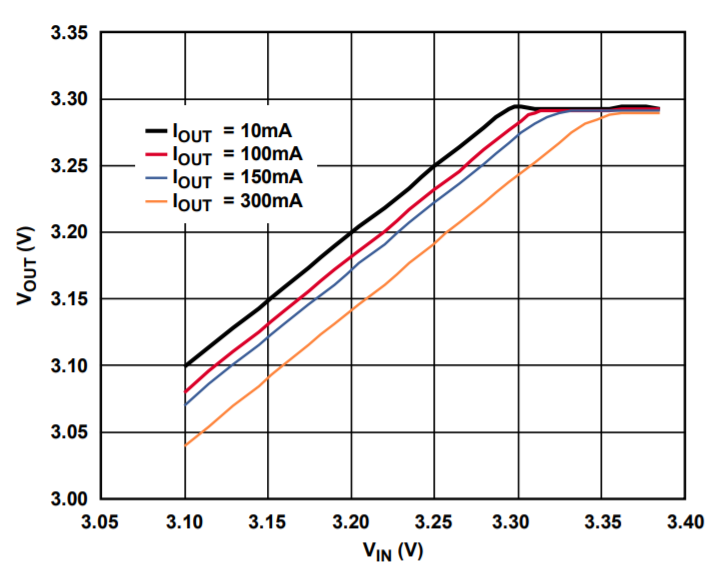
\includegraphics[width=120mm]{data/Linearregler_3_3V.png}
		\caption[ADP 122 Linearregler Spannungsverhalten]{Eingangsspannung vs. Ausgangsspannung \cite{ADP122LinearRegulator}} %picture caption
		\label{fig:Linearregler 3.3V}
	\end{center}
\end{figure} 

Für unsere Anwendung sind die mittleren zwei Kurven (rot und grau) interessant. Auffällig ist, dass bei $V_{ein}$<3.3V, die Abweichung zwischen $V_{ein}$ und $V_{aus}$ um ca. 0.025V unterscheiden. Die Abweichung $F_{error}$ ist somit kleiner 1$\%$.
\\
Nicht nur die Komponenten im Dojo selbst benötigen eine konstante Spannungsversorgung, sondern auch der Lade-IC während dem Ladevorgang. Da Der Ladevorgang mittels induktiver Ladung erfolgt, kann hierbei die Spannung extrem schwanken. Es wird also direkt nach der Sekundärspule und dessen Gleichrichtung ein Spannungsregler eingebaut. Hierbei wird ein MCP1703A der Firma Microchip verwendet. Dieser gibt bei einer maximalen Eingangsspannung von $16V_{DC}$, konstant $5V_{DC}$ ab. Der maximale Ausgangsstrom beträgt hierbei 250mA und ist somit für unsere Anwendung gut geeignet. Einen Einblick in das Spannungsregelverhalten gibt nachfolgende Abbildung \ref{fig:Linearregler 5V}.

\begin{figure}[H]
	\begin{center}
		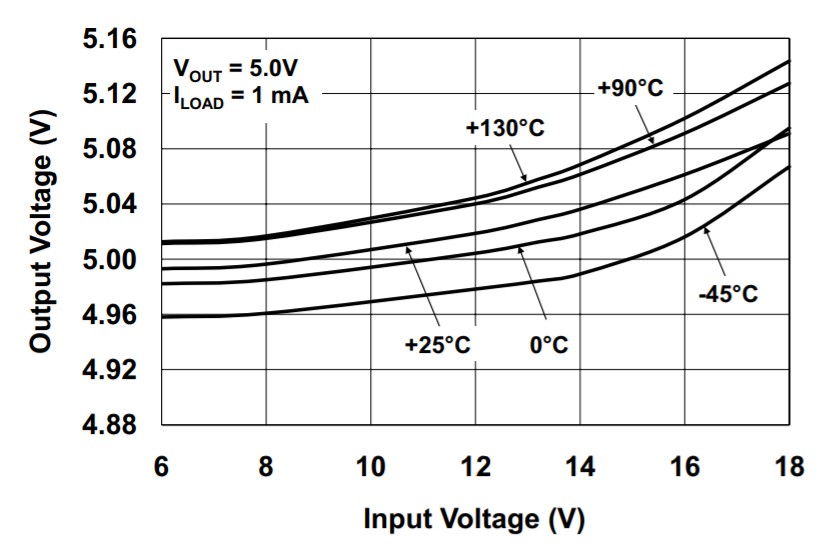
\includegraphics[width=120mm]{data/Linearregler_5V.png}
		\caption[MCP1703A Linearregler Spannungsverhalten]{Eingangsspannung vs. Ausgangsspannung \cite{MCP1703LinearRegulator}} %picture caption
		\label{fig:Linearregler 5V}
	\end{center}
\end{figure} 

Augenfällig ist, dass die Ausgangsspannungskurve im Bereich von 6V bis 16V (T=$25^\circ\text{C}$) rund 0.1V schwankt. Dies stellt jedoch keine Probleme für den Lade-IC dar, da dieser einen Eingangsspannungsbereich zwischen 3.75V bis 6V vorweist. Ebenfalls in der obigen Grafik ersichtlich ist die grosse Erwärmungstoleranz des Spannungsreglers. Dies ist aufgrund dessen wichtig, dass es durch die induktive Übertragung durchaus zu grosser Erwärmung in unmittelbarer Nähe kommen kann.

\subsubsection{Audioausgabe}
Die Funktionsweise des Knochenschallgebers wird hier kurz erläutert, sowie dessen Spezifikation (Versorgungsspannung, Ausgangsleistung etc.)


\subsubsection{Microcontroller}
Hier werden die Anforderungen an den Mikrocontroller aufgeführt, die Wahl begründet und auch das On-Chip Bluetoothmodul näher betrachtet.
